\chapter {Enterprise JavaBean Integration}
\section {Advantages of OpenCms \& EJB}
Running OpenCms in an application server environment provides facilities
for making use of distributed object architectures, particularly with
regard to Enterprise JavaBeans  technonolgy. Using these techniques,
processes behind the web site may be structured and distributed in a
component oriented way. Server sided presentation logic and business
logic can be developed strictly separated, according to the four-tier
architecture described in the J2EE Application Model: OpenCms takes care
of the presentation of the data, using the integrated template engine
and master templates for displaying it in a general layout, while the
generation of the content data is relocated to the EJB (figure~\ref{EJB}).

\begin{figure}[!hbt]
\begin{center}
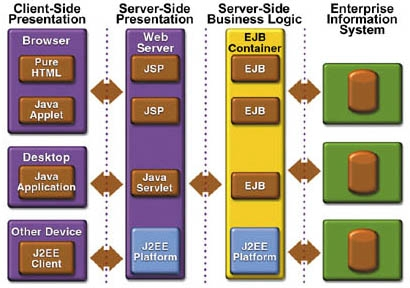
\includegraphics[clip,width=\sgw]{pics/ejb/ejb}
\end{center}
\caption[OpenCms and EJB]{OpenCms and EJB.}
\label{EJB}
\end{figure}

\index{EJB}
Implementing EJB components implicates a lot of advantages that enhance
the ease of handling with business data. This includes:

\begin {itemize}
\index{Concurrency}
\item {\bf Concurrency:}
The EJB server handles any concurrencies between EJB. The developer
doesn't have to care about threads or synchronization.
\index{Transactions}
\item {\bf Transactions:}
All set of tasks that have to be executed together will be managed by
the EJB server
\index{Persistence}
\item {\bf Persistence:}
The EJB server ensures, that any object is actually containing the most
recent data from any external database.
\index{Distributed Objects}
\item {\bf Distributed Objects:}
Clients do not have to know the exact location of Beans it is using.
This is transparent to the client. The EJB server takes care of  all
communication and remote method invocations (RMI).
\index{Naming}
\item {\bf Naming:}
The EJB server provides a service for looking up distributed objects.
This enables the client to request remote objects.
\index{Security}
\item {\bf Security:}
Authentication, access control and secure communications are ensured by
the server.
\end{itemize}

In the environment of OpenCms, EJBs may be used for different purposes,
such as plausibility checks of user input, database access or connection
to host systems. Even reuse of existing shared libraries is possible by
{\name "wrapping"} them with EJB components.

\section {EJB basics}
There are two different types of Enterprise Beans: Entity and Session
Beans. Entity Beans model real-life objects usually represented by some
records in a database. Session beans are used to map processes or tasks.
They usually operate on the data modelled by Entity Beans.
There is a further distinction between stateful Session beans, if the
Bean stores data over more than one session and stateless Session beans,
if the Bean only operates with the current parameters.
To implement an Enterprise Java Bean at least three components
are required:

\begin{itemize}
\index{Remote interface}
\item {\bf Remote interface:}
This interface contains all business methods that may be called remotely
(i.e. all methods visible from OpenCms). It has to extend EJBObject.

\index{Home interface}
\item {\bf Home interface:}
This one keeps all methods for finding, deleting or creating new EJB
objects. It must contain the create() Method for building new objects
and extends EJBHome.

\index{Bean class}
\item {\bf Bean class:}
This class implements all methods defined in the two interfaces above.
Note! Though the methods match the ones defined in the interfaces, these
are not implemented in this class.
For defining a entity bean, an additional component is required:

\index{Primary key}
\item {\bf Primary key:}
This is a class implementing a pointer to the database.
\end{itemize}

Since OpenCms only calls, but not implements EJB modules, only the two
interfaces become important at this point: They are essential for
looking up and calling an EJB.
Two sample home and remote interfaces may look as follows (these
examples are taken from the WebLogic {\name "examples" package)}:

\begin{java}
public interface TraderHome extends EJBHome \{\\
\jtaba  Trader create() throws CreateException, RemoteException;\\
\}\\

public interface Trader extends EJBObject \{\\
\jtaba  public  TradeResult buy (String stockSymbol, int shares)\\
\jtabb    throws RemoteException;\\

\jtaba  public TradeResult sell (String stockSymbol, int shares)\\
\jtabb    throws RemoteException;\\
\}\\
\end{java}


\section {Calling an EJB}
Calling an Enterprise JavaBean from OpenCms is quite easy and only
requires four steps:

\begin{enumerate}
\item   Get the {\name "initial context"}. Every Bean has a  initial context
object defining the Bean's environment containing the URL for the naming
service, the user and his password.
\item Get the EJB home. This is the implementation of the home
interface and can be used to get the EJB object.
\item Get the EJB object
\item Call any required EJB method on this object.
\end{enumerate}

In the Java code, this may look like:

\begin{java}
import javax.naming.Context;\\
import javax.naming.InitialContext;\\

Context jndiContext = getInitialContext();\\
TraderHome home = (TraderHome)jndiContext.lookup(C\_JNDI\_TRADER);\\
Trader t = home.create()\\
TradeResult res = t.buy("FFN", 100);\\
\end{java}

Instead of the buy() method every other method defined in the remote
interface could be called.
For getting the initialContext, some additional steps must be executed.
Note, that the name of the context factory is application server
dependend. This example again shows the code for the WebLogic server:

\begin{java}
protected Context getInitialContext() throws Exception \{\\
\jtaba     // Get an InitialContext\\
\jtaba     String factory = "weblogic.jndi.WLInitialContextFactory";\\
\jtaba     String url = "t3://localhost:7001";\\
\jtaba     Properties h = new Properties();\\
\jtaba     h.put(Context.INITIAL\_CONTEXT\_FACTORY, factory);\\
\jtaba     h.put(Context.PROVIDER\_URL, url);\\

\jtaba     // the following lines may be omitted,\\
\jtaba     // if no user authentication is required\\
\jtaba     h.put(Context.SECURITY\_PRINCIPAL, "system");\\
\jtaba     h.put(Context.SECURITY\_CREDENTIALS, "weblogic");\\

\jtaba     return new InitialContext(h);\\
\}\\
\end{java}

In Order to compile an OpenCms template class including EJB calls, some
additional import statements are required for making the EJB components
known to the class:

\begin{itemize}
\item {\bf javax.naming.*}. This will be needed to lookup an EJB component
using the initialContext. This package can be found in Sun's Java
2 SDK, Enterprise Edition (J2EE).
\item {\bf Home interface} for getting the EJB object
\item {\bf Remote interface}, since the EJB object will implement this.
\end{itemize}

\section{Refinements}
\subsection{Configuration}
It might be useful not defining the application server URL, user name
and password hard-coded in the Java class. Instead of this, these values
should be in an external properties file. You can use the
opencms.properties for this, which can be accessed using the method
{\meth getConfigurations} on the cms object.

Alternatively, a class can use it's own property file residing in the
server's file system (similar to the opencms.properties). The class

{\code source.org.apache.java.util.ExtendedProperties}

can be used for easily accessing this file.

\subsection{Error handling}
It is highly recommended to add an error and exception handling to an
EJB call. This avoids any server configuration error or EJB method
exception from being reflected to the calling OpenCms class. Otherwise
each non-caught exception inside the EJB component will probably cause a
strange result on the generated web page or even crash the calling
template class (the end user will see an "Internal Server Error" in his
browser).
Debugging will be very hard in this case because often the bug cannot be
located in the EJB immediately. Therefore the exception handling should
include a debugging output in the OpenCms log file by using the static
OpenCms.log() method.

The error handling should consider the following cases:

\begin{itemize}
\item Application server not reachable
\item Wrong user/password
\item EJB component not found (wrong JNDI name)
\item Method on EJB object not found (probably using wrong remote
interface)
\item EJB-Method throws an exception
\end{itemize}

In most of these cases, further generation of the current page will be
impossible since important data expected by the EJB is missing. Then, a
redirect to an error page can be initiated to inform the user, that the
server could not be processed.


